\documentclass[../sherrill-Mix_thesis.tex]{subfiles}
\begin{document}
\graphicspath{{im/}{intro/im/}}
\chapter{Introduction}
\section{The HIV epidemic}
	In 1981, physicians began to notice a mysterious increase, often clustered in men who had sex with men or intravenous drug users, in the occurrences of Kaposi's sarcoma and pneumocystis pneumonia \citep{Gottlieb1981,Friedman-Kien1981,Hymes1981,Masur1981,Siegal1981,Gottlieb1981a}. 
	
	Kaposi's sarcoma was, until 1981, a rare cancer in the US found largely in elderly men with Jewish or Mediterranean ancestry \citep{Laor1979}. Kaposi's sarcoma had also been seen in immunocompromised individuals \citep{Klein1974,Myers1974,Kapadia1977} and there were suggestions that it was a virus-associated cancer \citep{Safai1981} although the causative human herpesvirus would not be discovered for another decade \citep{Chang1994,Sitas1999}. 
	
	Pneumocystis pneumonia was known to be caused by infection of the alveoli with the yeast-like fungus \emph{Pneumocystis jirovecii} \citep{Burke1973,Hughes1977}. Pneumocystis pneumonia was almost exclusively seen only in patients with suppressed immune systems or immune disorders and rarely, if ever, in immunocompetent individuals \citep{Hughes1977}. %, previously known as \emph{Pneumocystis carinii} \citep{Stringer2009}

	The mechanism for this spike of opportunistic infections was clarified when researchers found severe T cells depletion and decreases in cellular immunity in these patients \citep{Masur1981,Siegal1981,Gottlieb1981a,Gerstoft1982,Masur1982}. This disease was eventually labeled acquired immunodeficiency syndrome (AIDS). However, the underlying cause remained unclear. 
	
	Potential transmissions by transfusion \citep{Ammann1982,Ehrenkranz1982,Poon1982}, injection drug use \citep{Masur1981,Masur1982,Greene1982}, maternal transmission \citep{OReilly1982} and both homosexual \citep{Fannin1982,Gerstoft1982} and heterosexual \citep{Masur1982,Harris1983} contact pointed towards an infectious agent. In 1983, a virus later named human immunodeficiency virus type 1 (HIV-1) was isolated from patient samples \citep{Barre-Sinoussi1983,Gallo1983,Popovic1984,Levy1984} and soon detected in most immunodeficient patients \citep{Gallo1984,Sarngadharan1984,Safai1984,Levy1984}. 

	Reports of AIDS and associated opportunistic infections in sub-Saharan Africa soon revealed widespread endemic infection \citep{Clumeck1983,Clumeck1984,VandePerre1984,Piot1984} and a great diversity of viruses \citep{Nkengasong1994,Louwagie1995,Vidal2000,Rambaut2001,Yang2001,Kalish2004}. Retrospective studies suggested that the virus had been present, at least sporadically, in Europe and the USA for decades \citep{Froland1988,Garry1988} and circulating for even longer in Africa \citep{Bygbjerg1983,Vandepitte1983,Clumeck1984,Nahmias1986,Zhu1998,Worobey2008}. Archived patient samples containing HIV-1 genome fragments from as early as 1959 were found in what is now Kinshasa, in the Democratic Republic of Congo \citep{Nahmias1986}. These samples showed extensive genome diversification already present in the 1960s, suggesting that HIV-1 had been circulating in humans for some time \citep{Zhu1998,Worobey2008}. Phylogenetic analyses adding in contemporary HIV-1 type M sequences estimated a most recent common ancestor in the early 1900s \citep{Korber2000,Salemi2001,Sharp2001,Yusim2001,Worobey2008,Faria2014}.
	
	A virus similar to HIV causing AIDS in monkeys was soon discovered in macaques \citep{Daniel195,Peeters1989} and many other primates \citep{Peeters2001}. HIV-1 appeared most similar to virus found in chimpanzees \citep{Peeters1989,Huet1990} and surveys of wild chimpanzees revealed a closely related simian immunodeficiency virus infecting chimpanzees in southeast Cameroon \citep{Gao1999,Keele2006,VanHeuverswyn2007}.
	
	The ancestor of HIV-1 was likely transmitted from a chimpanzee to a human, perhaps during harvesting of chimpanzees for food \citep{Bowen-Jones1999,Hahn2000,Peeters2002,Wolfe2004,Wolfe2005,Kalish2005}, in the forests of southeastern Cameroon then virus was transported down the Sangha River \citep{Sharp2008} to the city of Kinshasha, where the virus began its global spread \citep{Vidal2000,Vangroenweghe2001,Worobey2008,Faria2014}. A combination of social upheaval, increased mobility, urbanization and mass vaccination campaigns with unsterilized needles appear to have provided fuel for the growing epidemic \citep{Chitnis2000,deSousa2010,deSousa2012,Faria2014}. A virus appears to have been carried from Africa to Haiti in the 1960s, perhaps by workers returning home from an exchange program \citep{Piot1984,Vangroenweghe2001}, and into the US in the 1970s \citep{Gilbert2007} before being detected in the US in 1981. In the past 34 years, HIV-1 has spread to over 78 million people and caused over 35 million deaths \citep{UNAIDSCGA2014}.

	%siv cpz is itself a recombinate http://www.sciencemag.org/content/300/5626/1713.full
	
	%With a most recent common ancestor of HIV-1 M type estimated in the early 1900s \citep{Korber2000,Salemi2001,Sharp2001,Yusim2001,Worobey2008,Faria2014}. Zoonotic transmissions had probably occurred previously but a combination of social upheaval, mobilization, urbanization and mass vaccination campaigns with unsterilized needles appear to have provided fuel for the growing epidemic \citep{Chitnis2000,deSousa2010,deSousa2012,Faria2014}. The virus may have moved from Africa to Haiti in the 1960s and into the US in the 1970s \citep{Gilbert2007}. [[mention clade B in haiti and widespread but many more in africa and worldwide starburst]]

	%rare but present in 1978 in SF \citep{Echenberg1985} and NYC \citep{Stevens}
	%Antia 2003 Nature evolve in chain of transmission with R0<1


	%global epidemic ("transmission partners") \citep{Wertheim2014}

	%larder1993 multidrug resistant mutations in vitro

	In the early days of the epidemic, there were no tests to detect the virus, and no treatments.  The presence of the virus was often revealed by the onset of AIDS. Opportunistic infections \citep{Moore1996} and death usually followed soon after. The median survival time after diagnosis with AIDS was about 1 year \citep{Rothenberg1987,Vella1992}. 

	Isolation of the virus allowed the detection of the virus through assays of antibody response. Testing revealed that, from infection, patients had a median survival time of around a decade \citep{Lui1986,Deschamps2000,Harrison2010,CGAIDSIHIVS2000}. % and thus that the virus had an extremely long period of clinical latency with few specific symptoms while remaining infectious.
	
	In 1987, the successful trial of the reverse transcriptase inhibitor azidothymidine provided the first hope for treatment \citep{Fischl1987,Fischl1989,Volberding1990} but it soon became apparent that the fast mutation rate of HIV \citep{Hahn1986,Preston1988,Roberts1988,Mansky1995,Mansky1996,Abram2010,Achuthan2014} and strong selection by drug therapy could quickly create drug-resistant forms of virus in patients receiving single drug therapy \citep{Larder1989,Larder1989a,Land1990,Boucher1990,Richman1990,Richman1991,Fitzgibbon1992,Richman1994,Schuurman1995,Schmit1996}. Median survival time from AIDS diagnosis rose to only about 2 years with therapy \citep{Creagh-Kirk1988,Fischl1989,Moore1992,Vella1992}. 
	
	Additional antiretrovirals, again targeting reverse transcriptase, were developed \citep{Vella2012}. Sequential or alternating administration of different antiretroviral drugs did not greatly improve prognosis \citep{Kahn1992,Skowron1993,Abrams1994,deJong1994,Schmit1996a}. Simultaneous treatment with two reverse transcriptase inhibitor offered modest benefits but viral escape was still common \citep{Collier1993,Hammer1996,Eron1995,Saravolatz1996,Darbyshire1996}.

	Development of drugs targeting other stages of the HIV replication cycle allowed synergistic combinations of antiretroviral drugs \citep{Dornsife1991,Johnson1991,Cox1994,Feng2009,Jilek2012,Kulkarni2014}. The difficulty for HIV of evolving multiple drug resistant mutations \citep{Chow1993,Larder1995} meant that therapy using simultaneous combinations of drugs finally began to offer patients more hope of long term survival \citep{Collier1996,Hammer1997,Gulick1997,Montaner1998,Moore1999}. With early triple therapy, median survival times rose to 20 years \citep{AntiretroviralTherapyCohortCollaboration2009,Harrison2010}, rising to $\frac{2}{3}$ of uninfected life expectancy \citep{ATCC2008,Keiser2004} and finally approaching control populations with uninterrupted antiretroviral treatment \citep{vanSighem2010,Nakagawa2013,Johnson2013}. %but inflammation and drug toxicity, health care burden still a problem \citep{Deeks2013}

	%Testing for HIV revealed that from the time of infection with HIV, patients had a median survival time of about 10 years without antiretroviral therapy\citep{Deschamps2000,Harrison2010,CGAIDSIHIVS2000}. %In patients in Haiti treated for symptoms but not with antiretrovirals, the median time to AIDS was 5.2 years and to death was 7.4 years \citep{Deschamps2000}. Median time to death 7--12 years \citep{CGAIDSIHIVS2000}. %Many types of opportunistic infections and poor survival times \citep{Moore1996}. 4.5 years to AIDS in transfusions \citep{Lui1986}.
	%About 20 years life expectancy in HAART era \citep{AntiretroviralTherapyCohortCollaboration2009,Harrison2010} although catching late and cofounding factors can increase mortality \citep{AntiretroviralTherapyCohortCollaboration2009}

	 

	%2/3 life expectency in 2005 \citep{ATCC2008,Keiser2004}. Life expectancy of HIV patients receiving consistent antiretrovirals now approaches control population \citep{vanSighem2010,Nakagawa2013,Johnson2013} but inflammation and drug toxicity, health care burden still a problem \citep{Deeks2013}

	%moore1992 survive >900 days median if >150 CD4 baseline

	HIV rebounds quickly after cessation of therapy \citep{Cillo2014}
	%Sharp2001 HIV m n o three separate cpz
	Groups and subtypes?

	early establishment of latent infection \citep{Chun1998a} within 3 days \citep{Whitney2014}
	SAHA induces latent \citep{Contreras2009}
	new drug for latency disulfram \citep{Xing2011}
	modest induction of latent provirus \citep{Cillo2014}
	characterizing latent reservoir rare cells present in resting actice and macro \citep{Chun1997}

	%Kalish2004 recombination common before big spread

	%Gallo1983 was contaminated 
	
	%, a rare disorder in the US \citep{Safai1981} that had been seen associated with immunosuppression \citep{Klein1974,Myers1974,Kapadia1977}, and pneumocystis pneumonia, an infection previously reported only in individuals with compromised immune systems \citep{Burke1973,Hughes1977}, in otherwise healthy individuals, often men who have sex with men or intravenous drug users \citep{Gottlieb1981,Friedman-Kien1981,Hymes1981,Masur1981,Siegal1981,Gottlieb1981a}. , a rare tumor now known to be associated with a human herpesvirus \citep{Chang1994,Sitas1999}, and pneumocystis pneumonia, an opportunistic infections,  .  A severe T cells depletion and decrease in cellular immunity was observed in these patients \citep{Masur1981,Siegal1981,Gottlieb1981a,Gerstoft1982,Masur1982}. Potential transmissions by transfusion \citep{Ammann1982,Ehrenkranz1982}, injection drug use \citep{Masur1981,Masur1982,Greene1982} and both homosexual \citep{Fannin1982,Gerstoft1982} and heterosexual \citep{Masur1982,Harris1983} contact were soon observed.

	%The virus was isolated \citep{Barre-Sinoussi1983,Popovic1984,Gallo1984}

	%HIV2 \citep{Clavel1986}

	%First HIV antibody test \citep{Safai1984}

	%Origin in chimpanzee \citep{Gao1999}

\section{The HIV virus}
	HIV is an enveloped single strand positive-sense retrovirus, an RNA virus which uses reverse transcription to create a DNA intermediate in host cells \citep{Baltimore1970,Temin1970}. Viral encoded integrase protein discovered \citep{Grandgenett1978} and mapped to \threePrime{} end of pol \citep{Panganiban1984,Schwartzberg1984,Donehower1984} through mutation and loss of function.  Mutations at ends also results in defective viruses \citep{Panganiban1983}.

	\begin{figure}
		\centering
		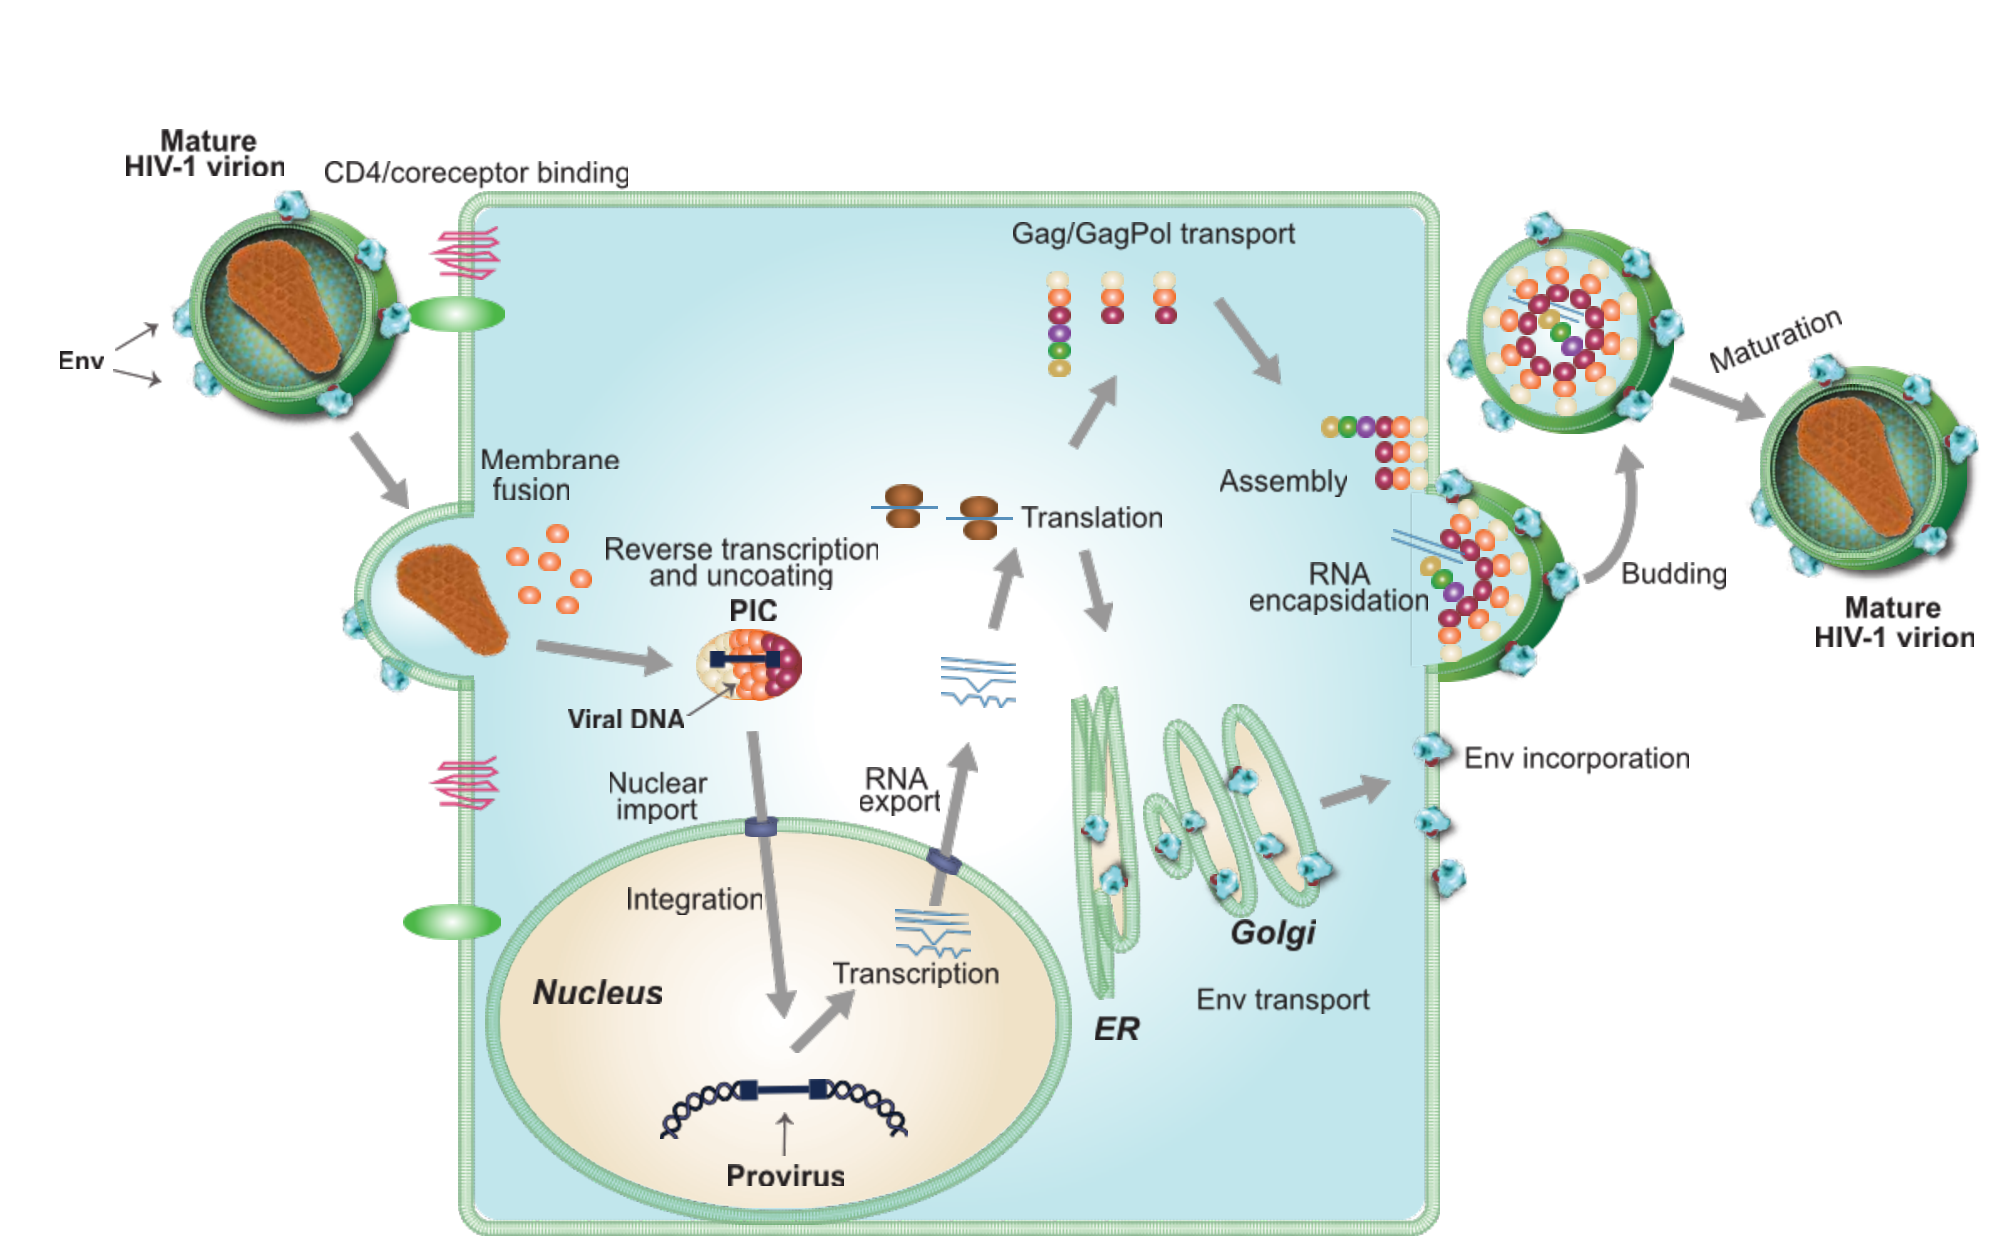
\includegraphics[width=\textwidth]{lifecycle.pdf}
		\caption[The HIV replication cycle]{The HIV replication cycle} %[[check rick book for caption]]
		\label{figHIVLifecycle}
	\end{figure}

	\begin{figure}
		\centering
		\floatbox[{\capbeside\thisfloatsetup{capbesideposition={right,top}}}]{figure}[\FBwidth]{
			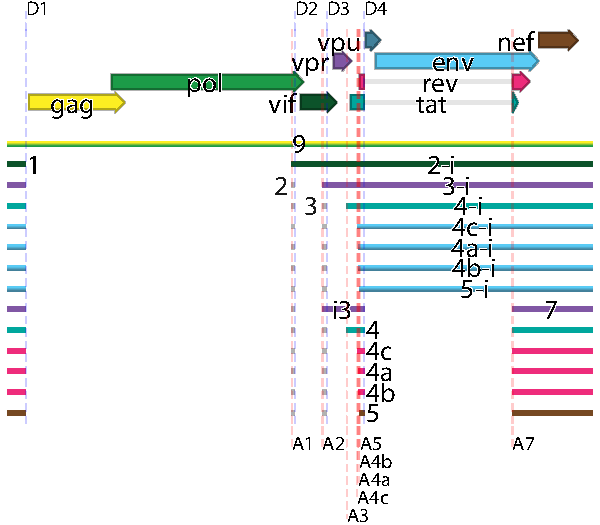
\includegraphics[width=.7\textwidth]{exonProt2.pdf}
		}{
			\caption[The HIV-1 genome]{The HIV-1 genome. Arrows indicate open reading frames. Dashed lines show major splice acceptors (red) and donors (blue). Major spliceforms are shown as thin rectangles and colored according to their corresponding open reading frame.}
			\label{figHIVGenome}
		}
	\end{figure}


	The HIV genome encodes genes for at least two polyproteins and seven proteins:\\ % \gag{} and \pol{}, and seven proteins, \tat{}, \rev{}, \nef{}, \vpr{}, \vif{} and \vpu{}.
	\begin{description}
		\item[\gag{}]
			Gag (group specific antigens) is a myristoylated membrane protein which is [[something]] on the virion surface and cleaved by viral protease after virion budding to produce matrix, capsid, nucleocapsid and p6 protein along with two small spacer peptides SP1 and SP2. 
			\begin{description}
				\item[MA]
					p17 MA (matrix) aids in transport of genome to the nucleus \citep{Heinzinger1994}.
				\item[CA]
						p24 CA (capsid) proteins assemble into to form a protective shell around RNA genome of the virus. The viral capsid is composed of around 1500 copies of CA arranged into hexameric rings interspersed with with 12 pentameric rings to form fullerene cone \citep{Ganser1999,Li2000,Byeon2009,Zhao2013}. CA binds cellular CPSF6 \citep{Lee2010}, cyclophilin A \citep{Thali1994,Gamble1996} the cyclophilin domain of RanBP2 \citep{Schaller2011}, perhaps to gain access to the nucleus \citep{Schaller2011,Ocwieja2011} and to avoid premature uncoating and exposure of the viral genome to innate immunity \citep{Rasaiyaah2013}.
				\item[NC]
					p7 NC (nucleocapsid)
				\item[p6]
					p6 (protein 6 kda) is a small protein which appears to primarily recruit cellular proteins to allow virion budding from the cell membrane \citep{Veronese1987,Goettlinger1991,Strack2003} and aid in the packaging of Vpr in to particles \citep{Paxton1993}.
			\end{description}
		\item[\pol{}]
			Pol (polymerase) is cleaved by viral protease to produce reverse transcriptase, RNaseH, integrase and HIV protease. 
			\begin{description}
				\item[RT]
					p51 RT (reverse transcriptase)
				\item[RNase H]
					p15 RNase H
				\item[IN]
					p31 IN (integrase) is a dimeric enzyme integrates the retroviral DNA into host chromatin \citep{Bushman1990,Engelman1991,Panganiban1984,Maertens2010,Hare2010}. Integrase removes two nucleotides from from \threePrime{} ends of the viral DNA and inserts the pair of viral ends into host DNA \citep{Bushman1991}.
				\item[PR]
					PR (protease) is a dimeric aspartyl protease \citep{Wlodawer1989} that cleaves viral polyproteins Gag and Pol \citep{Kraeusslich1989,Kohl1988}. 
			\end{description}
		\item[\env{}]
			gp160 Env is a trimeric transmembrane protein that mediates entry through fusion of viral and cellular membrane by binding its receptor \cdFour{} \citep{Dalgleish1984,Klatzmann1984,Lifson1986,Lifson1986a,Maddon1986} and coreceptors CXCR4 \citep{Feng1996} CCR3 and CCR5 coreceptor \citep{Choe1996,He1997}. gp160 is cleaved into two subunits gp41 and gp120 \citep{Veronese1985} by cellular furin protease \citep{Hallenberger1992}. The envelope protein is highly glycosylated to form a `glycan shield' against adaptive immune response \citep{Wei2003}. There are about 14 Env proteins per virion \citep{Zhu2006}. Env is highly variable within and between patients \citep{Holmes1992,Shankarappa1999} due to positive selection from host immune recognition \citep{Bonhoeffer1995,Wolinsky1996,Ross2002}. %positive selection at same sites over time correlate with slower progression \citep{Wolinsky1996,Ross2002} 1\% distance increase diversity in env per year (decreases later in infection) \citep{}
		\item[\tat{}]
			Tat (transactivator) protein is a transactivator of expression from the HIV-1 long terminal repeat \citep{Sodroski1985,Sodroski1985a,Cullen1986}. Virus does not replicate efficiently without this transactivation \citep{Dayton1986}. and appears to regulate cellular expression such as downregulation of major histocompatibility complex type I expression \citep{Howcroft1993}.  Tat may suppress miRNA silencing pathway \citep{Bennasser2005,Triboulet2007,Qian2009} but controversial \citep{Lin2007}.
			%http://www.sciencemag.org/content/260/5112/1320.abstract6
		\item[\rev{}]
			Rev (regulator of expression of virion proteins) trans-activator protein shuttles between the nucleus and cytoplasm \citep{Meyer1994} and causes the export of partially spliced and unspliced viral transcripts \citep{Sodroski1986,Feinberg1986,Knight1987,Malim1988,Gutman1988} from the nucleus through recognition of a structured RNA rev response element \citep{Malim1989,Malim1989a}.
		\item[\nef{}]
				Nef (negative factor) is a myristoylated membrane associated protein \citep{Yu1992} that is involved in multiple functions. Nef causes endocytosis of the HIV receptors CD4 \citep{Garcia1991,Benson1993,Aiken1994,Lama1999,Ross1999} and CCR5 \citep{Michel2005} and viral surveillance major histocompatibility complex molecules \citep{Schwartz1996,Collins1998,Stumptner-Cuvelette2001,Blagoveshchenskaya2002}. Nef also induces T cell activation through interactions with signaling kinases and the T cell receptor \citep{Xu1999,Schrager1999,Wang2000,Simmons2001,Schrager2002}. In contrast, Nef in most other primate lentiviruses inhibits activation and inflammation \citep{Schindler2006} perhaps indicating that the gain of \vpu{} in HIV-1 and its simian relatives allowed the loss of the immune inhibition traits of \nef{} and contributes to the increased pathogenecity in these viruses \citep{Kirchhoff2008,Kirchhoff2009}.
		\item[\vpr{}]
			Vpr (viral protein R) is a 15 kDa protein \citep{Wong-Staal1987,Cohen1990} with diverse functions that is incorporated into virions \citep{Cohen1990a,Yuan1990}. Vpr arrests the cell in the G2 phase of the cell cycle \citep{Jowett1995,Re1995,He1995,Rogel1995,Noronha2001} and aids in transport of the viral genome to the nucleus \citep{Heinzinger1994}. Vpr also appears to trans-activate viral expression \citep{Goh1998,Subbramanian1998} and induce apoptosis \citep{Stewart1997,Shostak1999} but these may be linked to conditions caused by cell cycle arrest.
		\item[\vif{}]
			Vif (virion infectivity factor) counteracts the cellular restriction factor APOBEC3G \citep{Sheehy2002} by excluding APOBEC3G from incorporation into the virion \citep{Mariani2003} and causing APOBEC3G to be ubiquitinated and degraded \citep{Sheehy2003,Marin2003,Yu2003}. APOBEC3G is otherwise packaged into virions \citep{Harris2003} and deaminates the HIV genome during reverse transcription causing G-to-A hypermutation \citep{Harris2003,Mangeat2003,Zhang2003,Lecossier2003}.
		\item[\vpu{}]
			Vpu (viral protein U) \citep{Cohen1988,Strebel1988} is a small integral membrane protein which has two known functions; degradation of CD4 and downregulation of BST-2 from the cell membrane [[cites]]. Vpu causes cellular CD4 to be ubiquitinated and degraded \citep{Willey1992,Bour1995} which prevents interactions between progeny virus Env and host cell CD4 \citep{Marshall1992,Lama1999,Ross1999,Cortes2002} and superinfection by other viruses \citep{Benson1993}  while also releasing Env proteins from CD4 interactions in the endoplasmic reticulum \citep{Crise1990,Bour1991}. Vpu also counteracts the cellular restriction factor BST-2, which would otherwise interfere with viral budding \citep{Neil2008}. Vpu does not appear to be found in the virion \citep{Strebel1989}.
			%cd4 degradation 
	\end{description}

	In Chapter \ref{chapPacBio}, we look for spliceforms potentially encoding more proteins and find two new proteins.
	%http://www.sciencedirect.com/science/article/pii/S0966842X04000253


	%CD4 receptor \citep{Lifson1986,Lifson1986a,Maddon1986} CXCR4 \citep{Feng1996} CCR3 and CCR5 coreceptor \citep{Choe1996,He1997} classification \citep{Berger1998}
	HIV tropism infects macrophages \citep{Koenig1986}

	%pre integration complex \citep{Bowerman1989}. extracts from HIV infected cells able to integrate in cell free system \citep{Ellison1990,Farnet1990} contains integrase and matrix and RT \citep{Farnet1991,Bukrinsky1993} %farnet1991 says int only
	%integrase alone can integrate HIV DNA\citep{Busman1990}

	%long terminal repeats at each end \citep{Hughes1978}. integrates in many locations \citep{Hughes1978}


	%nobels prophage \citep{Lwoff1966} provirus \citep{Temin1976} %dna complementary to rna \citep{Neiman1972} and DNA from RSV transformed cells can transform cells \citep{Hill1972}.
	%JThe virus was sequenced in 1985 \citep{Wain-Hobson1985,Muesing1985,Ratner1985,Sanchez-Pescador1985}.

	%Splice classes \citep{Muesing1985} and others?

	HIV diversification within a single patient in env loop \citep{Holmes1992} positive selection \citep{Bonhoeffer1995,Ross2002} positive selection at same sites over time correlate with slower progression \citep{Wolinsky1996,Ross2002} 1\% distance increase diversity in env per year (decreases later in infection) \citep{Shankarappa1999}

	%REWORD THIS Highly active antiretroviral therapy (HAART) can suppress HIV-1 replication in infected patients, but the ability of HIV to persist as an inducible reservoir of latent proviruses \citep{Chun1995, Chun1997,Wong1997,Finzi1999, Davey1999,Hamlyn2012,Stoehr2013} obstructs eradication of the virus and functional cure \citep{Richman2009}. These latent proviruses are long lived \citep{Finzi1999,Siliciano2003} and relatively invisible to the immune system \citep{Finzi1997,Chun1997}.

	half life of 2 days and $10^9$ CD4 T cells per day \citep{Ho1995,Wei1995,Perelson1997}
	macrophages? half life 1--4 weeks \citep{Perelson1997,Lambotte2000,Zhu2002} 
	resting CD4 T cells\citep{Finzi1997,Chun1997,Wong1997}

	Retrovirus package two copies of RNA in each virion \citep{Bellamy1974,Kung1975,Kung1976}. Interstrand transfer during the reverse transcription step allows recombination \citep{Panganiban1988,Hu1990,Hu1990a}
	[[strand transfer rt refs 3--5 in \citep{Panganiban1988}]]

\section{Integration and latency}
	Integration into a host chromosome is an integral step in the retrovirus replication cycle.

	cells can produce virus without cell death in vitro \citep{Hoxie1985}
	first latent HIV \citep{Folks1986}
	High throughput integration site sequencing \citep{Schroder2002,Wang2007} %schroder is sanger


\section{HIV splicing}
	RNA splicing was first observed in adenovirus \citep{Berget1977,Chow1977}. Improved understanding of HIV and other viruses offers medical benefits. Although HAART treatments have greatly improved HIV prognosis, long-term survival of HIV patients remains reduced by at least a decade compared to the general population \citep{Lohse2007}. In addition HAART does not provide a permanent cure \citep{Richman2009} and the long-term costs of treatment runs into hundreds of thousands of dollars over the lifetime of a patient \citep{Hutchinson2006,Schackman2006}.  Induction or alteration of splicing has been suggested as a potential treatment \citep{Fukuhara2006,Mandal2010} and differential splicing appears to be one factor limiting cross species infection and the development of animal models of HIV \citep{Zheng2003}. 

	Rev balanced with weak 3' splice sites \citep{Kammler2006}.

	Splicing changes due to splice factor changes in macrophages \citep{Dowling2008}

	Driven by a strong selective pressure for genome compactness \citep{Gelinas1986,Herman1987,Shin2000}, HIV and other lentiviruses subvert host cell alternative splicing pathways to allow tight packing of their genetic information. Through weak splice sites and overlapping reading frames (Figure \ref{figHIVGenome}), the virus manages to produce precise quantities of at least nine proteins and polyproteins from its single transcription start site and less than 10 kb genome \citep{Stoltzfus2009}. 

	As such an integral part of the virus life cycle\citep{Kim1989,Pomerantz1990}, alteration of splicing poses a tempting therapeutic target. Inhibition of cellular splicing factors reduces viral reproduction in many genome-wide siRNA screens \citep{Brass2008,Konig2008,Bushman2009} and several members of the spliceosome interact with viral proteins in affinity pulldowns \citep{Jager2012}. Open reading frames in uncharacterized transcripts appear to produce epitopes useful for vaccine development \citep{Bansal2010}. Potential treatments altering viral splicing through small molecule inhibitors \citep{Fukuhara2006,Bakkour2007} and gene therapy \citep{Asparuhova2007,Mandal2010} have restricted viral replication \emph{in vitro}. However without methods to quantify viral splicing or a thorough quantification of splicing under varying conditions, the development of such treatments remains limited. 

	Viral proteins also interact with components of the cellular splicing complex \citep{Tange1996,Berro2006,Jager2012}. These interactions have been reported to change splicing in viral\citep{Berro2006,Bohne2007,Jablonski2010} and cellular transcripts \citep{Kuramitsu2005,Hashizume2007} and raise the possibility that the virus has evolved to alter host splicing. A genome-wide study of changes in cellular splicing during HIV infection would greatly clarify this hypothesis but no such study has been performed. 

	Alternative splicing, the differential inclusion of exons and removal of introns from primary mRNA transcripts, allows rapid evolution of protein segments \citep{Kopelman2005,Xing2005,Su2006} and drastic increases in the number of proteins generated by a single DNA sequence \citep{Watson2005}. Many viruses subvert the splicing machinery of their eukaryotic hosts to modify their viral mRNA \citep{Pollard1998}. 

	In particular, it has previously been reported that HIV utilizes alternative splicing to generate more than 40 mRNA transcripts encoding at least 9 proteins and polyproteins from a genome smaller than 10kb \citep{Purcell1993}. A specific progression of viral transcripts appear in the cytoplasm of the host cell as infection progresses allowing a shift from regulatory protein production in early infection into virion production in late infection \citep{Kim1989,Pomerantz1990,Klotman1991}. Because HIV has only a single transcription start site, these transcriptional changes are driven by alternative splicing \citep{Stoltzfus2009}. 

	 Although it plays such an essential role for the virus, only a single detailed census of viral splicing has been reported \citep{Purcell1993}. Due to limitations in technology, this study was limited to only the most abundant transcripts in lab-adapted HIV strains in cell culture \citep{Purcell1993}. Yet rare transcripts may play an important role in immune response \citep{Bansal2010} and encode unknown proteins \citep{Benko1990}; lab adapted HIV can differ markedly from viruses actually found in patients \citep{Fujita1992};  cell cultures often do not reflect \emph{in vivo} conditions \citep{McAllister1971}; and splicing can vary between humans \citep{Kwan2007,Hull2007} and cell types \citep{Wang2008,Barash2010}. Without a fuller characterization of transcripts under these relevant conditions, many aspects of viral splicing will remain poorly understood.

	Alternative splicing may also play an unappreciated role in HIV-host interactions. Viral proteins interact with the splicing complex \citep{Tange1996,Berro2006,Jager2012} and alter splicing of some cellular transcripts \citep{Kuramitsu2005,Hashizume2007}. Yet, although infection has been shown to cause genome-wide changes in the expression of cellular genes \citep{Vahey2002,Wout2003,Mitchell2003,Rotger2010,Chang2011}, no genome-wide study of cellular alternative splicing during HIV infection has ever been reported. Such a genome-wide study of splicing changes might reveal a distortion of diverse cellular splicing which is adaptively advantageous to the virus. 

	Current sequencing advancements allow a much broader and deeper investigation of viral splicing. Targeted amplification with RainDance droplet PCR offer the potential to reduce size bias inherent in bulk PCR \citep{Tewhey2009}. RNA-seq with Illumina sequencing allows extremely deep sequencing of cellular and viral transcripts with billions of bases of short read sequence \citep{Marioni2008,Morin2008}. Single molecule sequencing with Pacific Biosciences provides reads approaching 20,000 bases \citep{Eid2009,Schaefer2012} that could characterize entire viral transcripts in one continuous read. By combining these technologies, viral and cellular transcripts could be interrogated to an unprecedented level.

	A better understanding of viral splicing and viral effects on host splicing may bring therapeutic benefits. siRNA inhibition of splicing factors reduces HIV replication in many genome-wide screens \citep{Brass2008,Konig2008,Bushman2009}. Alteration of viral splicing through small molecule inhibitor of SR protein kinases\citep{Fukuhara2006} and Splicing Factor 2 \citep{Bakkour2007}, shRNA against spliceosomal U7 snRNP \citep{Asparuhova2007} and expression of modified spliceosomal U1 snRNP \citep{Mandal2010} show treatment potential \emph{in vitro}. In addition, rare uncharacterized HIV transcripts and their encoded proteins appear to produce potent immune response in HIV patients \citep{Bansal2010} thus offering potential targets for vaccine development. Yet without methods to characterize viral RNA and measure the effects of treatments on viral splicing, further development is inhibited. 

	Inclusion and exclusion of a particular stretch of RNA into an mRNA is determined by a balance of RNA secondary structure \citep{Buratti2004,Jablonski2008,Shepard2008}, chromatin structure \citep{Allo2009}, nucleosome positioning \citep{Tilgner2009}, histone marks \citep{Schwartz2009}, previous splicings \citep{Crabb2010}, order of intron removal \citep{Takahara2002,Mata2010} and enhancers \citep{Zahler1993} and suppressors \citep{Smith2000} that bind specific motifs \citep{Ule2006}. Together these factors create a precise controllable splicing code \citep{Barash2010,Xiong2011,Witten2011}.  

	 In HIV, splicing occurs between at least four splice donors and eight splice acceptors \citep{Stoltzfus2009}. Two splice donors, D1 and D4, are relatively strong while the remaining donors and all acceptors are fairly weak \citep{O'Reilly1995}. Several exonic splicing silencers \citep{Amendt1994,Levengood2012} and exon splicing enhancers \citep{Caputi2004,Asang2008} and a single intronic splicing silencer \citep{Tange2001} in the viral genome interact with many human splicing factors, including hnRNPs A1 \citep{Tange2001, Levengood2012} H, F, 2H9, and A2 \citep{Jablonski2008} and SR proteins SRp40\citep{Caputi2004,Tranell2010}, SRp75 \citep{Tranell2010}, ASF/SF2 \citep{Caputi2004} and SC35 \citep{Jablonski2008}, to alter viral splicing \citep{Stoltzfus2006,Stoltzfus2009}.

	Several viral proteins affect mRNA abundances. Rev causes export of unspliced viral mRNA that would otherwise be trapped in the nucleus \citep{Legrain1989} to be exported \citep{Fischer1994,Pollard1998} and may also interact with splicing factors to alter viral splicing \citep{Tange1996}. The HIV protein Tat is best known for its transactivation of viral transcription \citep{Sodroski1985,Jones1994} and triggering apoptosis in uninfected cells \citep{McCloskey1997,Campbell2004} but Tat also appears to independently affect alternative splicing of viral transcripts\citep{Berro2006,Bohne2007,Jablonski2010,Miller2011}. Viral protein Vpr is known to cause cell cycle arrest \citep{Rogel1995} and mediate nuclear import of the viral preintegration complex \citep{Fouchier1998}. Vpr also appears to alter alternative splicing of some cellular transcripts \citep{Kuramitsu2005,Hashizume2007} and interact with the SMN complex \citep{Jager2012}, which assembles spliceosomal snRNP \citep{Gubitz2004}. Although all three of these proteins modify viral splicing, whether they also cause widespread alterations in cellular splicing is unknown.

	Despite the critical role alternative splicing plays in viral replication, no genome-wide studies of lentiviral effects on cellular splicing or  detailed censuses of viral alternative splicing in biologically relevant settings have been published.

	RNA-seq offers a much broader view of alternative splicing than previously possible \citep{Trapnell2010,Rogers2012} but Illumina sequencing has not yet been applied to the study of differential splicing in host RNA of HIV-infected cells. There have been many studies of cellular expression using microarrays \citep{Vahey2002,Wout2003,Mitchell2003,Rotger2010,Miller2011} and Sage \citep{Ryo1999,Lefebvre2011} but only a single study using Illumina RNA-seq and alternative splicing changes were not reported \citep{Chang2011}. Thus a potentially significant aspect of HIV-host interactions remains unknown.

	The most extensive survey of HIV transcripts to date was published in 1993\citep{Purcell1993}. Technology at the time necessitated the use of Northern blots and RNA protection assays \citep{Purcell1993} which can not distinguish multiple similarly sized transcripts or detect rare transcripts. This study also focused on a single lab adapted \hivNL{} strain in HeLa cell culture.

	Many previous studies of viral splicing have used lab-adapted strains of HIV which often differ from patient isolates \citep{Fujita1992} in cell cultures which often differ from primary cells \citep{McAllister1971}. Selection under cell culture conditions may quickly alter splicing patterns to down regulate proteins unneeded \emph{in vitro}.  Characterization of alternative splicing in biologically relevant cell types infected with clinical isolates of HIV are sorely needed.


	%

\section{Host cell interactions}
%HIV may suppress miRNA silencing pathway \citep{Bennasser2005,Triboulet2007,Qian2009} but controversial \citep{Lin2007}
%TAR-dervied miRNA might change gene expression particularly apoptosis pathway \citep{Klase2009}.

%Interferon inducible genes
%change splicing factors \citep{Zhu2002,Dowling2008}

%repetitive elements and vaccination

\section{HIV detection}
%http://www.medscape.com/viewarticle/715166_2
	Immunoassays provide cheap immediate testing of HIV infection in patients. These tests are based on the enzyme-linked immunosorbent assay (ELISA), using an enzyme linked to an antibody to produce a detectable signal in the presence of antigen \citep{Yalow1960,Engvall1971,VanWeemen1971}. %If the labeled antibodies are targeted to human antibodies then a patient's immune response to an antigen can be measured.
	
	The isolation of HIV \citep{Barre-Sinoussi1983,Gallo1983,Popovic1984,Levy1984} allowed the production of large quantities of virions. These virions were bound to a substrate, sera from patients added and any patients antibodies sensitive to HIV allowed to bind. Any unbound antibodies were washed away. Then a peroxidase enzyme-labeled antibody targeted to human antibody bound was added, allowed to bind and the unbound antibodies again washed away. Any HIV-targeted patient antibodies would bind the antigen and be bound in turn by the peroxidase-labeled antibody and the peroxidase would then change the color of media \citep{Safai1984,Sarngadharan1984,Ward1986}. These tests had a large false positive rate and the standard procedure was to perform multiple ELISA tests follow by a Western blot test \citep{Towbin1979,CDC1985} but false positives were still prevalent \citep{Burke1986}. More conservative criteria and cleaner lab procedures reduced false positives \citep{Burke1988}. These assays have been developed to fourth generation \citep{Chappel2009} with more sensitive and specific detection of patient antibodies and earlier detection using antibodies against the HIV capsid protein \citep{Weber1998,Weber2002}.  

	Slightly less specific but rapid immunoassays providing results in 30 minutes have been developed to allow point-of-care testing with many fewer patients lost to follow up prior to delivery of results \citep{Kassler1995,CDCP1998,CDCP2002}. Rapid tests detecting HIV in oral fluids have been developed and obviate the need for a blood draw \citep{Gallo1997,Delaney2006,SemaBaltazar2014}. These rapid care tests allow self testing at home \citep{Granade2004,PantPai2013}.

	Reverse transcription and PCR amplification offers another alternative \citep{Hart1988,Ou1988} but is not currently cost effective for primary patient screening \citep{Long2011}.

	Tests allowing point-of-care qualitative HIV detection are now widespread but point-of-care assays for viral load in a patient exist. In addition, existing laboratory-based tests are relatively expensive and require specialized equipment making access difficult in resource-limited settings \citep{Fiscus2006,Wang2010a}. Without viral load measures, \cdFour{} T cell counts or clinical presentation are used to infer the emergence of drug. These criteria are not specific or sensitive enough without viral load measures so many patients are unnecessarily switched to second line therapy \citep{Mee2008,VanOosterhout2009} or switched too late leading to accumulations of drug resistant mutations \citep{Hosseinipour2009}.  In Chapter \ref{chapLamp}, we design loop-mediated isothermal amplification methods that can be used with microfluidics to create a point-of-care assay of infection and viral load in resource-limited settings.

\section{Contribution summaries}
	Much of this work was performed as part of a large collaboration. It would not tell a complete story in isolation. Therefore, I have preserved the chapters in published form and detailed my contribution to each project at the start of the chapter.


\end{document}
